\chapter{Исследование и построение решения задачи}

Как и для любой другой задачи машинного обучения, для решения поставленной задачи можно выделить следующие типичные подзадачи:\\

\begin{enumerate}
\item Выбор признакового описания; \\
\item Выбор метода классификации;\\
\item Выбор набора данных;\\
\item Выбор метрики для валидации;\\
\end{enumerate}

Рассмотрим каждый этап и принятые на нём решения по отдельности.

\section{Получение признакового описания объектов}

\subsection*{Формальное описание решаемой задачи}

Мы решаем задачу бинарной классификации. Пусть $X$ - множество описаний объектов, $Y$ - конечное множество меток классов. Существует неизвестная целевая зависимость --- отображение $y^*\colon X \rightarrow Y$, значения которой известны только на объектах конечной обучающей выборки $X^m = \{(x_1, y_1),\dots,(x_m, y_m)\}$. Требуется построить алгоритм $a\colon X \rightarrow Y$, способный классифицировать произвольный объект $x \in X$. Признаком называется отображение $f\colon X \rightarrow D_f$, где $D_f$ --- множество допустимых значений признака.

Для базовой модели используется такая же, как и в статье \cite{yuanInsiderThreatDetection2018b}, схема получения признакового описания. Она состоит в описании каждого отдельного уникального действия пользователя соответствующим уникальным среди всех возможных действий номером. Для каждого отдельного дня каждого отдельного пользователя составляется последовательность действий, при этом последовательности малой длины отбрасываются. Перед подачей на вход модели используется one-hot кодирование номеров действий, которая заключается в том, что каждому числу $i$ ставится в соответствие вектор. В этом векторе элемент с индексом $i$ равен 1, а все остальные элементы равны 0. Вектор имеет размерность максимального значения, которое может иметь число на входе.

Таким образом, для данной задачи, $X=(D_{f})^L$, где каждый объект обозначает последовательность действий одного пользователя в течение одного дня. $L$ обозначает фиксированную длину всех последовательностей, а $D_{f}$ --- множество допустимых значений описания одного действия за день. $D_f$ является конечным множеством чисел, где каждое число обозначает один уникальный тип действия, который можно совершить (отправить письмо в нерабочее время со своего устройства, просмотреть файл в рабочее время с чужого устройства и т. д.). Присваиваемые значения действиям не несут сами по себе смысла, кроме специального значения $0$, который требуется для увеличения коротких дневных последовательностей до требуемого значения $L$. $Y=\{0,1\}$, где $1$ обозначает наличие вредоносного поведения за день, а $0$ --- его отсутствие.

% 

% Отдельным важным вопросом стоит извлечение полезных для классификаторов признаков. Если когда-то для этого требовался кропотливый ручной труд исследователя, то сейчас нейросети способны выполнить эту задачу в автоматическом режиме и при условии достаточно большого набора данных способны выделить достаточно полезные признаки для последующих моделей. По этой причине в \cite{yuanInsiderThreatDetection2018b}, перед подачей данных классификатору, они проходят черед LSTM-сеть, которая играет роль кодировщика данных. Поэтому и в данной работе используется обученный отдельно LSTM-кодировщик.

Кроме того, можно расширить количество разновидностей действий с помощью дополнительных признаков, таких как роль сотрудника в организации и количественные суммарные характеристики (например, количество отправленных писем). \\

\subsection*{Генерация дополнительных признаков}

 Потенциально полезным направлением для генерации дополнительных признаков, является использование контента рабочих файлов. Данный аспект набора данных CERT зачастую не используется в большинстве современных работах. Но в то же время при генерации контента авторы неявным образом составляют для каждого пользователя уникальную смесь интересующих его тематик. И подразумевается, что нехарактерная смена интересов пользователей, может служить сигналом об аномальности его поведения. Поэтому использование контента пользователя, представленного в виде набора тематик, имеет большой потенциал для улучшения качества конечного классификатора.\\
Добавление контента можно формально описать как расширение признакового описания объектов. Каждому отдельному тексту соответствует набор тематик $(p_1, \dots p_m)$, где $p_i$ - вероятность i-ой тематики, а $m$ - количество рассматриваемых тематик. Таким образом, каждый объект будет описываться вектором $x = (n, (p_1, \dots p_m))$, где $n$ - номер вида совершаемого действия. Если у действия нет контента (например, это действие подключение устройства), то $p_i = 0, \forall i$.\\

\begin{itemize}
\item Признак роли сотрудника. Имеет очевидный смысл, что для разных ролей сотрудников характерны различные паттерны поведения (например, техподдержка намного чаще имеет доступ к сторонним машинам).
\item Контентные признаки. В наборе данных CERT контент сгенерирован методом ``мешок слов'', где слова последовательности сгенерированы по неявно заданным тематикам пользователей. Полезно при анализе действий пользователя также учитывать тематики, с которыми он работает. Резкая смена тематик пользователя может свидетельствовать об аномальности его поведения.\\
Выделения тематик из контента может производиться двумя алгоритмами NMF и LDA.
\end{itemize}

\section{Выбор метода классификации}

По обзору моделей становится понятна проблема отсутствия единого бенчмарка. Большинство рассмотренных работ используют набор данных CERT, но каждая работа отличается схемой валидации результатов и валидационной метрикой. Пусть даже они используют один и тот же набор данных, это делает прямое сопоставление результаты различных работ довольно затруднительным. Однако следует выделить работу \cite{yuanInsiderThreatDetection2018b}, так как в ней заявлены наилучшие реалистичные результаты и хорошо описаны подробности реализации, что упростит воспроизведение результатов. В выбранной работе не использовались контентные данные, которые можно использовать для улучшения результатов модели.\\

На этом этапе мы пытаемся достичь похожих результатов, описанными авторами.\\
Поскольку в архитектуре решения отдельно обучаются две части модели, имеет смысл валидировать кодировшик также и на более простых классификаторах, чтобы исключить влияние качества самого свёрточного классификатора. Для этого возьмём алгоритмы логистической регрессии, SVM, случайный лес, бустинг и одноклассовый KMeans.
\\
В силу большого объема набора данных, также следует использовать алгоритмы понижения размерности PCA и NMF. PCA взят в силу своей линейности и простоты, NMF взят потому, что он может дополнительно извлечь полезные признаки и улучшить качество моделей.\\

LSTM и CNN модели обучаются по отдельности. LSTM обучается как речевая модель, где роль ``слов'' играют отдельные действия пользователя, а ``предложением'' является последовательность действий за день. Формально, это можно описать как задачу обучения без учителя (unsupervised), где для каждой подпоследовательности действий с индексами от $0$ до $i$ предсказывается следующее действие с индексом $i+1$.\\
Каждое действие кодируется, как описано в базовой работе, с помощью one-hot кодирование.\\

\subsection{Улучшения}

Когда мы добились похожих результатов, мы должны улучшить качество работы системы. Для этого нам нужно собрать различные гипотетические варианты улучшения, обучить с ними модель и сравнить их с базовой моделью.\\
Так как реализуемое решение состоит из двух отдельных моделей, все потенциальные улучшения классификации можно разделить на две группы группы: улучшения для LSTM-кодировщика и улучшения для CNN-классификатора.
\subsection{Улучшения для LSTM-кодировщика}
\begin{itemize}
	\item Увеличение числа эпох.\\
	В оригинальной статье авторы обучали LSTM-кодировщик всего 10 эпох. При этом, было обнаружено, что после 10 эпох функция потерь продолжает падать как на тренировочной, так и на валидационной подвыборке. Было увеличено количество эпох до 200, когда функции потерь практически прекращают уменьшаться.\\
	\item Добавление Embedding-слоя\\
	Техника Embedding-слоя состоит в сопоставлении каждому отдельному токену (точнее, его индексу) собственному вектору малой размерности. Можно также считать Embedding-слой частным случаем линейного слоя, где индексы неявно one hot кодируются. Эта техника пользуется очень большой популярностью в сфере обработки естественных языков, так как она позволяла значительно улучшить качество работы для последующих задач.\\
	Самый простой вариант реализации - добавить Embedding-слой и обучать его вместе с обучением кодировщика. Веса этого слоя инициализируются случайно.\\
	Популярной техникой получения embedding'ов является word2vec \cite{mikolovEfficientEstimationWord2013a}. Её смысл заключается в обучении отдельной модели, называемой SkipGram, которая пытается для каждого токена в корпусе пытается предсказать ближайшие слова вокруг.\\
	Была реализована модель SkipGram, которая обучается на начальном наборе данных действий пользователя. Из последовательностей действий, которые разбиты по пользователям и датам, после сортировки по пользователям и датам составляется единая цельная последовательность, которая образует ``текст''. Эта последовательность подается на вход SkipGram для обучения.\\

% написать про изменение лосса

	После получения embedding'ов, они загружаются в соответствующий слой кодировщика. Далее, было испробовано два варианта обучения - статический и динамический, в которых мы либо замораживаем веса для этого слоя или нет.

% ссылку на статью, откуда это подсмотрено

	\item Добавление Attention-слоя.\\
	Как было отмечено в обзоре существующих решений, Attention имеет очень большой потенциал для улучшения качества работы кодировщика. На данном этапе, это улучшение не реализовано\\
	\item Написание собственной метрики точности, которая не игнорирует метки-пробелы.\\
	Это улучшение было сделано, чтобы улучшить интерпретируемость результатов обучения LSTM-кодировщиков.\\
	Функция потерь на валидационном наборе является хорошей мерой, чтобы сравнивать различные конфигурации кодировщиков друг с другом. Но проблема в отсутствии ясно интерпретации конкретных значений функции потерь.
	
	Точность, в свою очередь, является интуитивной метрикой, но её проблема состоит в том, что она не сильно отличается для разных обученных моделей. Это происходит потому, что большая часть всех меток занимают метки-пропуски, которые ставятся в конец малых последовательностей, чтобы все последовательности имели одинаковую длину. Так как все модели кодировщиков достаточно просто обучаются обнаруживать такие метки, точность становится очень большой.
	
	Чтобы решить эту проблему, была реализована собственная метрика, которая игнорирует заданные метки. Таким образом, скорректированная точность для обученных кодировщиков составляет около 77\%, что намного менее оптимистично по сравнению с обычной точностью и позволяет лучше понимать реальное качество работы кодировщика.
	
\end{itemize}
\subsection{Улучшения для CNN-классификатора}
\begin{itemize}
\item Взвешенная функция потерь. При обучении классификатора становится очевидно, что с некоторой эпохи модель начинает серьезно переобучаться. Так как переобучение может возникнуть из-за несбалансированности классов для борьбы с возникшей проблемы, при вычислении функции потерь, мы сильней штрафуем модель за ошибки в малом классе. Идея данного подхода и схема вычисления весов для каждого класса была взята из статьи \cite{yueImbalancedMalwareImages2017a}, где также решалась похожая задача с сильном нарушении баланса классов.\\
\item Добавления слоёв batch-нормализации. Популярной техникой в борьбе с переобучением в сверточных классификаторах является использование слоёв batch-нормализации, основанные на статье \cite{ioffeBatchNormalizationAccelerating2015}.\\
% Кратко описать, что есть батч-нормализация
Добавление этих слоёв после сверточных слоёв и перед функциями активаций сделало переобучение намного более слабо выраженным, но финальное качество модели изменилось не сильно. Комбинация взвешивания функции потерь и слоёв batch-нормализации, позволяет за малое число эпох достичь хорошей метрики на валидации.
\item Добавление слоёв Dropout. Другой популярной техникой борьбы с переобучение нейросетей является применение слоёв Dropout, представленные в статье \cite{srivastavaDropoutSimpleWay}. Суть этих слоёв заключается в том, что каждое значение предыдущего слое с заданной вероятностью оставляется таким же, либо приравнивается нулю. В свёрточных нейронных сетях эти слои ставятся после свёрточных слоёв, после функции активации.
\item Добавление weight decay (``Распад весов''). Является формой L2 регуляризации нейронных сетей во время этапа оптимизации.
\end{itemize}

% Кратко описать, что есть weight decay
% Написать про lr_annealing

\section{Выбор набора данных}

Из обзора набора данных, можно сделать вывод, что наборы данных поведенческой информации пользователей, имеют главный недостаток - малое количество данных, относительно потребностей для современных моделей машинного обучения. На этом фоне очень хорошо выделяется набор данных CERT, который имеет очень большой объём данных - как контекстных, так и контентных. Другим важным преимуществом набора данных CERT является наличие разметки вредоносного поведения, что также позволит нам использовать supervised модели.\\
Нетрудно увидеть, почему он пользуется большой популярностью среди исследователей и является де-факто бенчмарком. Поэтому для решения поставленной задачи разумно взять именно этот набор данных. Выбор набора данных CERT также позволит напрямую сравнивать результаты работы обученных моделей с результатами из других работ.

В случае выбранной темы, исходя из обзоров имеющихся наборов данных и существующих решений, разумно сделать выбор в пользу набора данных CMU CERT. Этот набор данных имеет множество преимуществ в виде, большого размера и наличия разметки различных видов зловредного поведения пользователей. Более того, этот набор данных является де-факто стандартом в моделировании инсайдерских атак, что даёт возможность напрямую сравнивать результаты своей работы с результатами других исследователей.\\
Также, исходя из этого, разумно выбрать версию набора данных 4.2, так как она наиболее часто исследуется. Также, как и в прочих работах, мы будем игнорировать различные классы зловредного поведения и будем рассматривать задачу бинарной классификации, где ``1'' обозначает некоторое зловредное поведения, а ``0'' - нормальное поведение.\\
CERT 4.2 является ``плотным'' набором данных, то есть он обладает нереалистично высоким количеством зловредных действий. Однако, для моделей, которые рассматривают каждого пользователя отдельно, это обстоятельство не должно влиять на результаты работы.

Набор данных CERT имеет пять файлов:
\begin{itemize}
	\item \textit{Logon.csv} --- вход и выход в систему
	\item \textit{Device.csv} --- подключение внешних устройств
	\item \textit{File.csv} --- операции с файлами
	\item \textit{Email.csv} --- электронная почта
	\item \textit{Http.csv} --- посещенные веб-сайты
\end{itemize}

Файлы \textit{File.csv}, \textit{Email.csv} и \textit{Http.csv} также имеют контентые данные  в виде набора предложений сгенерированных  по неявным тематикам пользователя.

После предобработки получено 329.845 последовательностей, сделанных за день каким-либо пользователем. Только 1293 (0.392\%) последовательностей содержат в себе зловредное поведение. 30\% (98.953) от объектов используется для валидации. Остальные 70\% последовательностей используются для обучения моделей.

\section{Выбор метрики для валидации}
Результаты обученной модели имеют мало смысла при отсутствии адекватной метрики. Поэтому важно сразу решить, какая метрика будет использовать при измерении качества работы на валидационной выборке данных.\\
Следует отметить, что выбранный набор данных имеет проблему несбалансированности классов - нормальное пользовательское поведения значительно больше представлено, чем аномальное. Поэтому, необходимо подбирать метрики исходя из этого. Такие метрики как Accuracy, Precision и Recall явно не подходят, потому что они не сбалансированны, хотя они могут быть полезны в качестве вспомогательных метрик, чтобы можно было понять, какого рода ошибки совершает модель. В то же время, среднее гармоническое метрик Precision и Recall (называемое F1-мерой) является устойчивой к несбалансированным наборам данных, что делает эту метрику адекватной.\\
Другим очень важным требованием к выбираемой метрике является популярность среди работ других исследователей. Это явлется необходимым условием для того, чтобы можно было напрямую сравнивать результаты работ.\\
Исходя из этого, самой адекватной метрикой является AUC ROC. Важным его преимуществом является независимость от выбранного порога бинаризации предсказании - метрике важно лишь то, что предсказания имеют корректный порядок по отношению к истинной разметке. Также изучение ROC-кривой может использоваться для анализа качества работы модели.\\
Эти качества делают данную метрику очень популярной для задач бинарной классификации, и данный случай не является исключением.\\
Также очень важным является то обстоятельство, что эта же метрика была выбрана и в работе \cite{yuanInsiderThreatDetection2018b}, которая была взята за основу. Это позволит напрямую сравнивать качество предсказаний.

\section{Результаты экспериментов}

Результаты экспериментов с классификаторами представлены в \autoref{tab:model_results}. Для CNN классификаторов представлен наилучшие результаты для разных комбинаций гиперпараметров.

\begin{table}[H]
\centering
\begin{tabular}{ |p{6cm}||p{3cm}|p{3cm}| }
 \hline
 \rowfont{\scriptsize}%
 \textbf{Эксперимент} & \rowfont{\scriptsize}\textbf{тренировочный ROC AUC} & \rowfont{\scriptsize}\textbf{валидационный ROC AUC}\\
 \hline\hline
 \rowfont{\normalsize}%
CNN & 0.9754 & 0.9566\\
CNN-weighted & 0.9902 & 0.9570 \\
CNN-batchnorm & 0.9984 & 0.9523\\
CNN-batchnorm-weighted & 0.9896 & 0.9530\\
СNN-content & 0.9438 & 0.9021 \\
CNN-dropout & 0.9669 & \textbf{0.9574} \\
\hline
PCA+SVM-linear & 0.480751 & 0.444866\\
PCA+SVM-poly3 & 0.767566 & 0.612348\\
PCA+SVM-rbf & 0.783510 & 0.637761\\
PCA+SVM-sigmoid & 0.544269 & 0.612614\\
\hline
NMF+SVM-linear & 0.870198 & 0.822704\\
NMF+SVM-poly3 & 0.818726 & 0.657016\\
NMF+SVM-rbf & 0.884946 & 0.679365\\
NMF+SVM-sigmoid & 0.572091 & 0.619073\\
\hline
LogisticRegression & 0.974562 & 0.908483 \\
PCA+LogisticRegression & 0.941257 & 0.906489 \\
NMF+LogisticRegression & 0.938370 & 0.908969 \\
\hline
KMeans & 0.852188 & 0.795787 \\
PCA+KMeans & 0.846038 & 0.785732 \\
NMF+KMeans & 0.898865 & 0.881201 \\
\hline
PCA+RandomForest & 0.999797 & 0.944633 \\
NMF+RandomForest & 0.995474 & 0.933625 \\
\hline
\end{tabular}
\caption{Результаты экспериментов с различными классификаторами.}
\label{tab:model_results}
\end{table}

``weighted'' обозначает взвешенную функцию потерь, ``batchnorm'' - применение слоёв batch-нормализацииь, ``content'' - добавление контентных данных, ``dropout'' - добавление Dropout-слоя. Также в таблице представлены эксперименты с прочими алгоритмами классификации. ``SVM-linear'', ``SVM-poly3'', ``SVM-rbf'' и ``SVM-sigmoid'' обозначает SVM с различными ядрами: линейное, полином третьей степени, радиальное и сигмоидное соответственно. PCA и NMF обозначают соответствующие алгоритмы понижения размерностей, которые применялись перед подачей данных на вход классификаторам. \\
KMeans, который применялся для экспериментов является одно-классовым. Фактически, алгоритм вычислял расстояние объекта до центроиды всего тренировочного набора данных. Также была попытка применения One-Class-SVM, но так как алгоритм может предсказывать только метки классов, а не их вероятности, то метрика AUC ROC не сильно отличалась от 0.5 для различных порогов.\\

Для всех экспериментов с обучением сверточной нейроной сети использовалась техника Early Stopping (ранняя остановка), при которой обучение модели прекращается только при условии остановки роста качества. В данном случае, обучение останавливается, если последние 20 эпох не было улучшение качества. Эта техника позволяет сократить количество эпох обучения моделей, которые уже не смог получить качество лучше при дальнейшем обучении.

Для CNN-классификаторов применялись различные наборы гиперпараметров: скорость обучения, размер weight decay, типы нелинейности в функциях активации (ReLU, LeakyReLU, гиперболический тангенс, ELU), наличие слоёв Dropout и Batch Normalization, размер весов для разных классов, Weight Decay (метод регуляризации весов модели для оптимизаторов), различные постоянные величины для скорости обучения и применение уменьшающейся скорости обучения.\\

На \autoref{fig:run-waves} показаны результаты переборы. Каждая кривая обозначает отдельный эксперимент и её цвет обозначает размер итоговой валидационной метрики, чем светлее кривая - тем больше метрика.

\begin{figure}[ht]
\noindent\makebox[\textwidth]{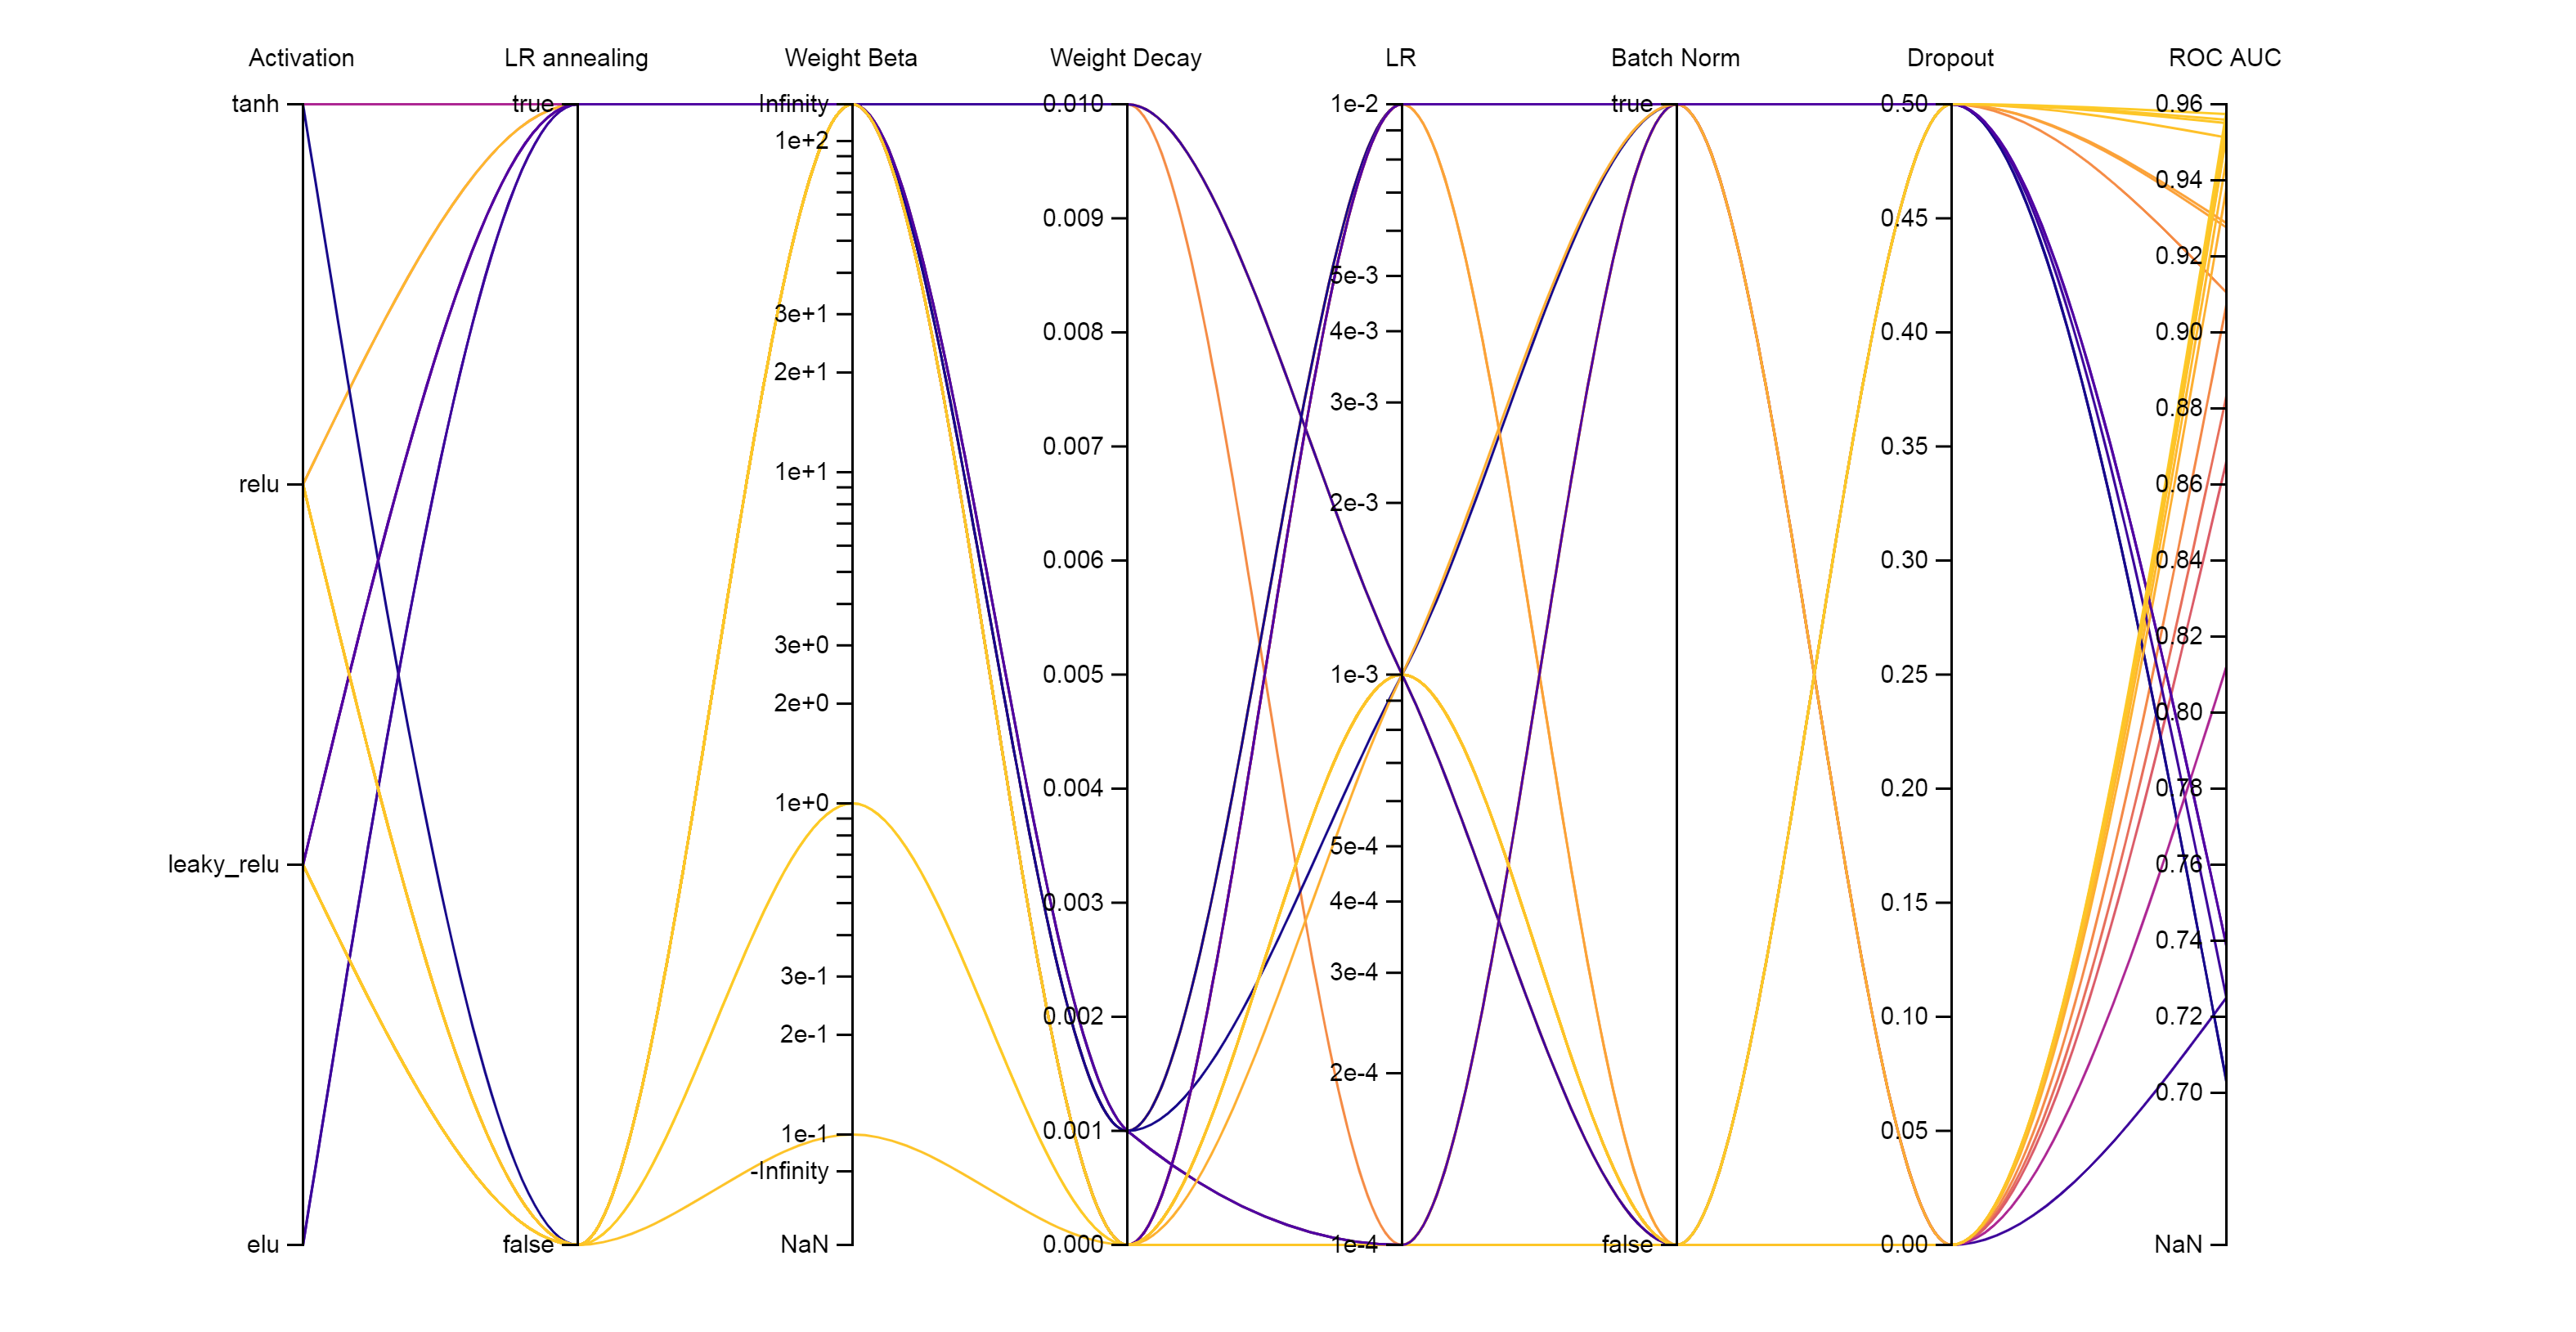
\includegraphics[width=\linewidth]{Section-0-Panel-0-5f4lnfvjk}}
\caption{Результаты экспериментов с различными гиперпараметрами}
\label{fig:run-waves}
\end{figure}

При переборе всех возможных наборов гиперпараметров валидационное качество не смогло значительно улучшиться. Однако, применение слоёв Batch Normalization и Dropout, а также взвешенных классов, помогают ускорить обучение модели без значительной потери валидационного AUC ROC. Как видно на \autoref{fig:batch-norm}, модели в среднем значительно раньше достигают своего пика, хотя и начинают намного раньше переобучаться, что характеризуется падением качества.
Также можно хорошо пронаблюдать эффект от добавления Dropout слоя на \autoref{fig:dropout}. Модель начинает медленее сходиться, но при этом модель не переобучается с резким падением качества. При добавлении этого слоя уменьшается разрыв между качеством на тренировочной и валидационной подвыборках.

\begin{figure}[h]
\noindent\makebox[\textwidth]{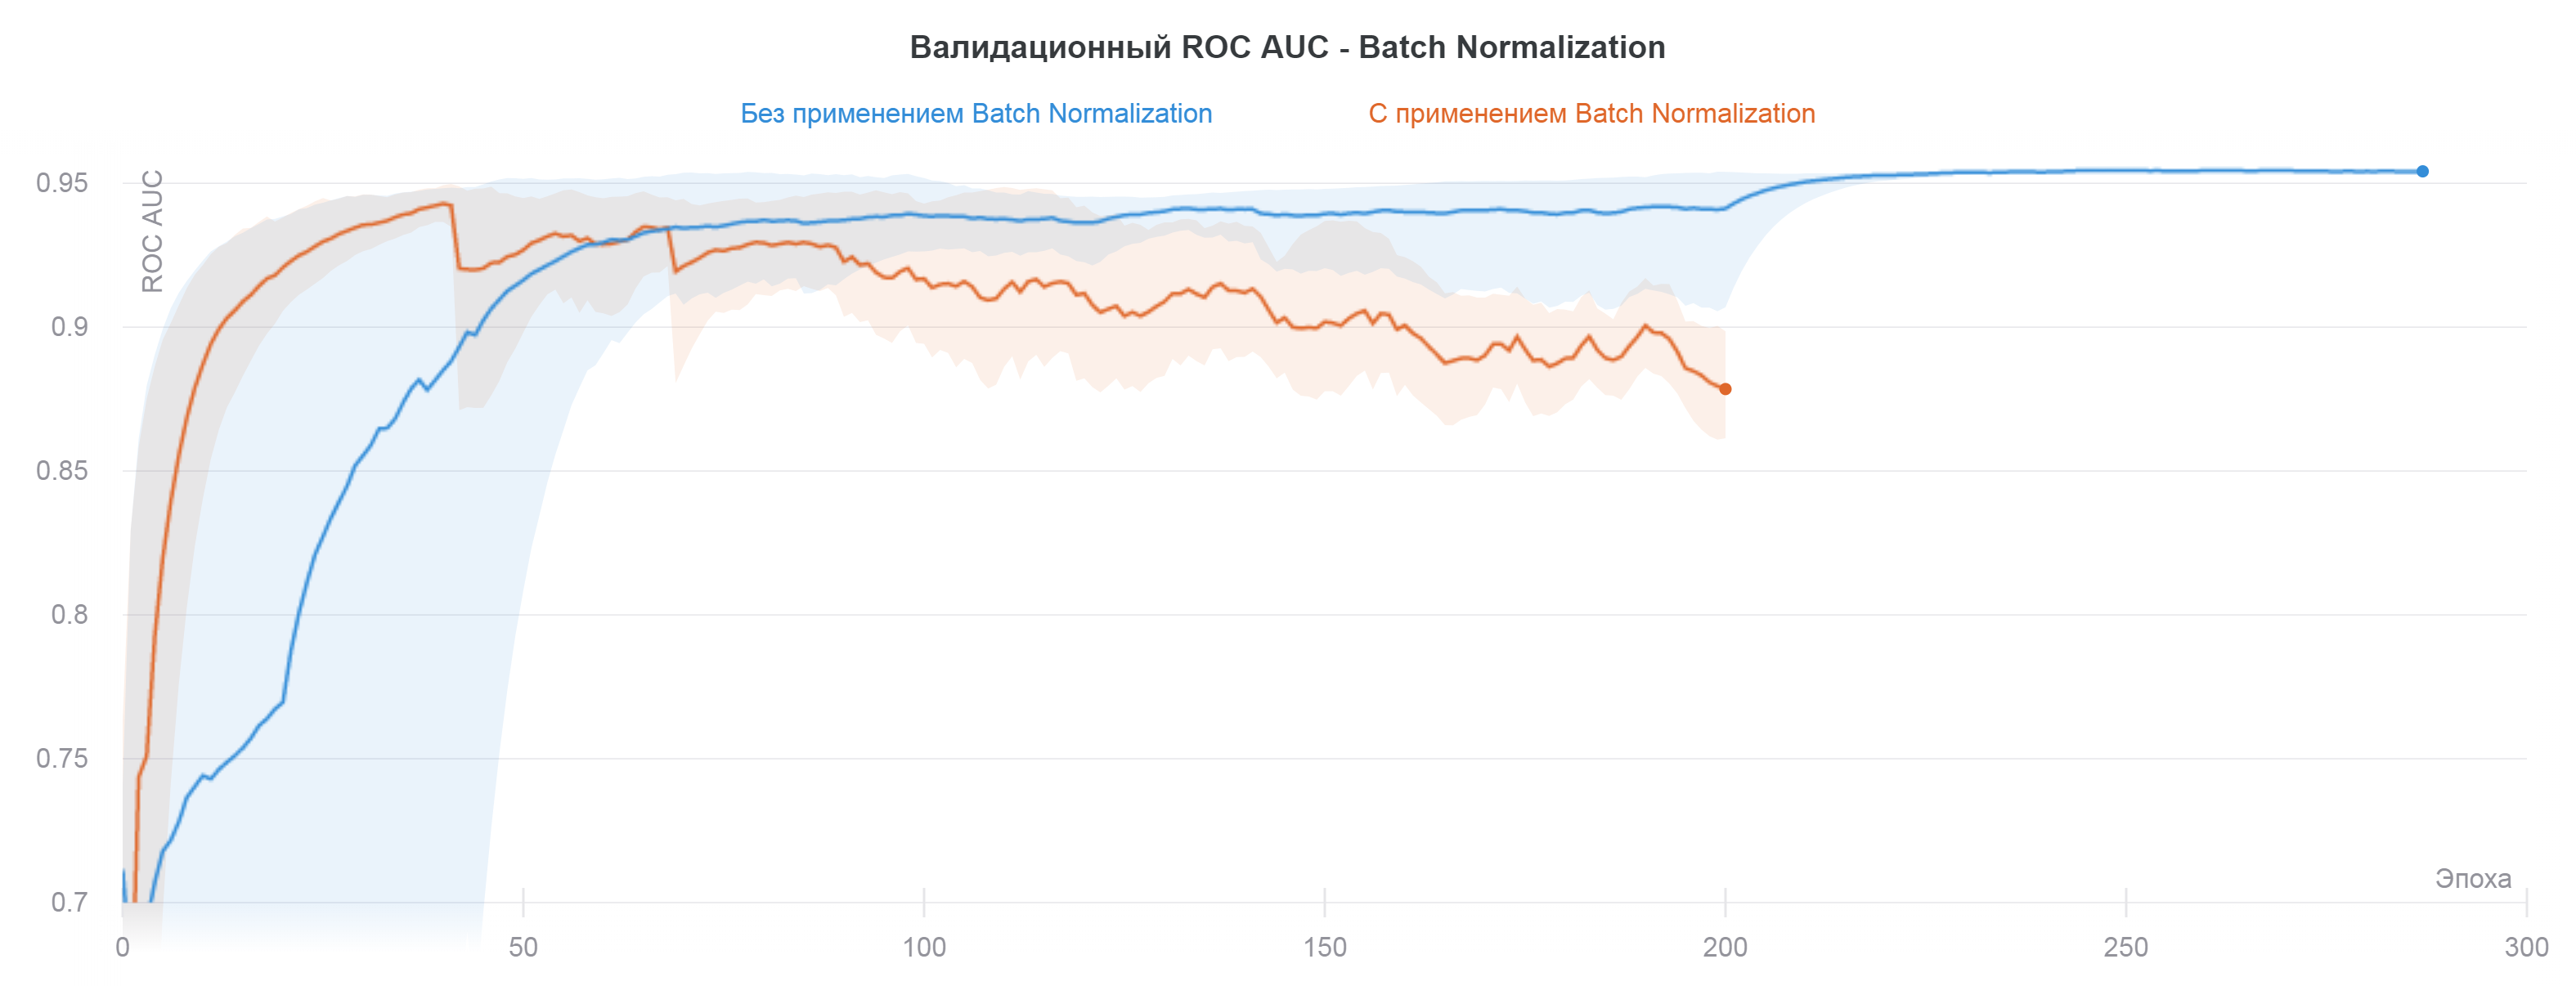
\includegraphics[width=\linewidth]{Section-0-Panel-2-wdsj85igb}}
\caption{Сравнение экспериментов с и без применения слоя Batch Normalization}
\label{fig:batch-norm}

\end{figure}
\begin{figure}[h]

\noindent\makebox[\textwidth]{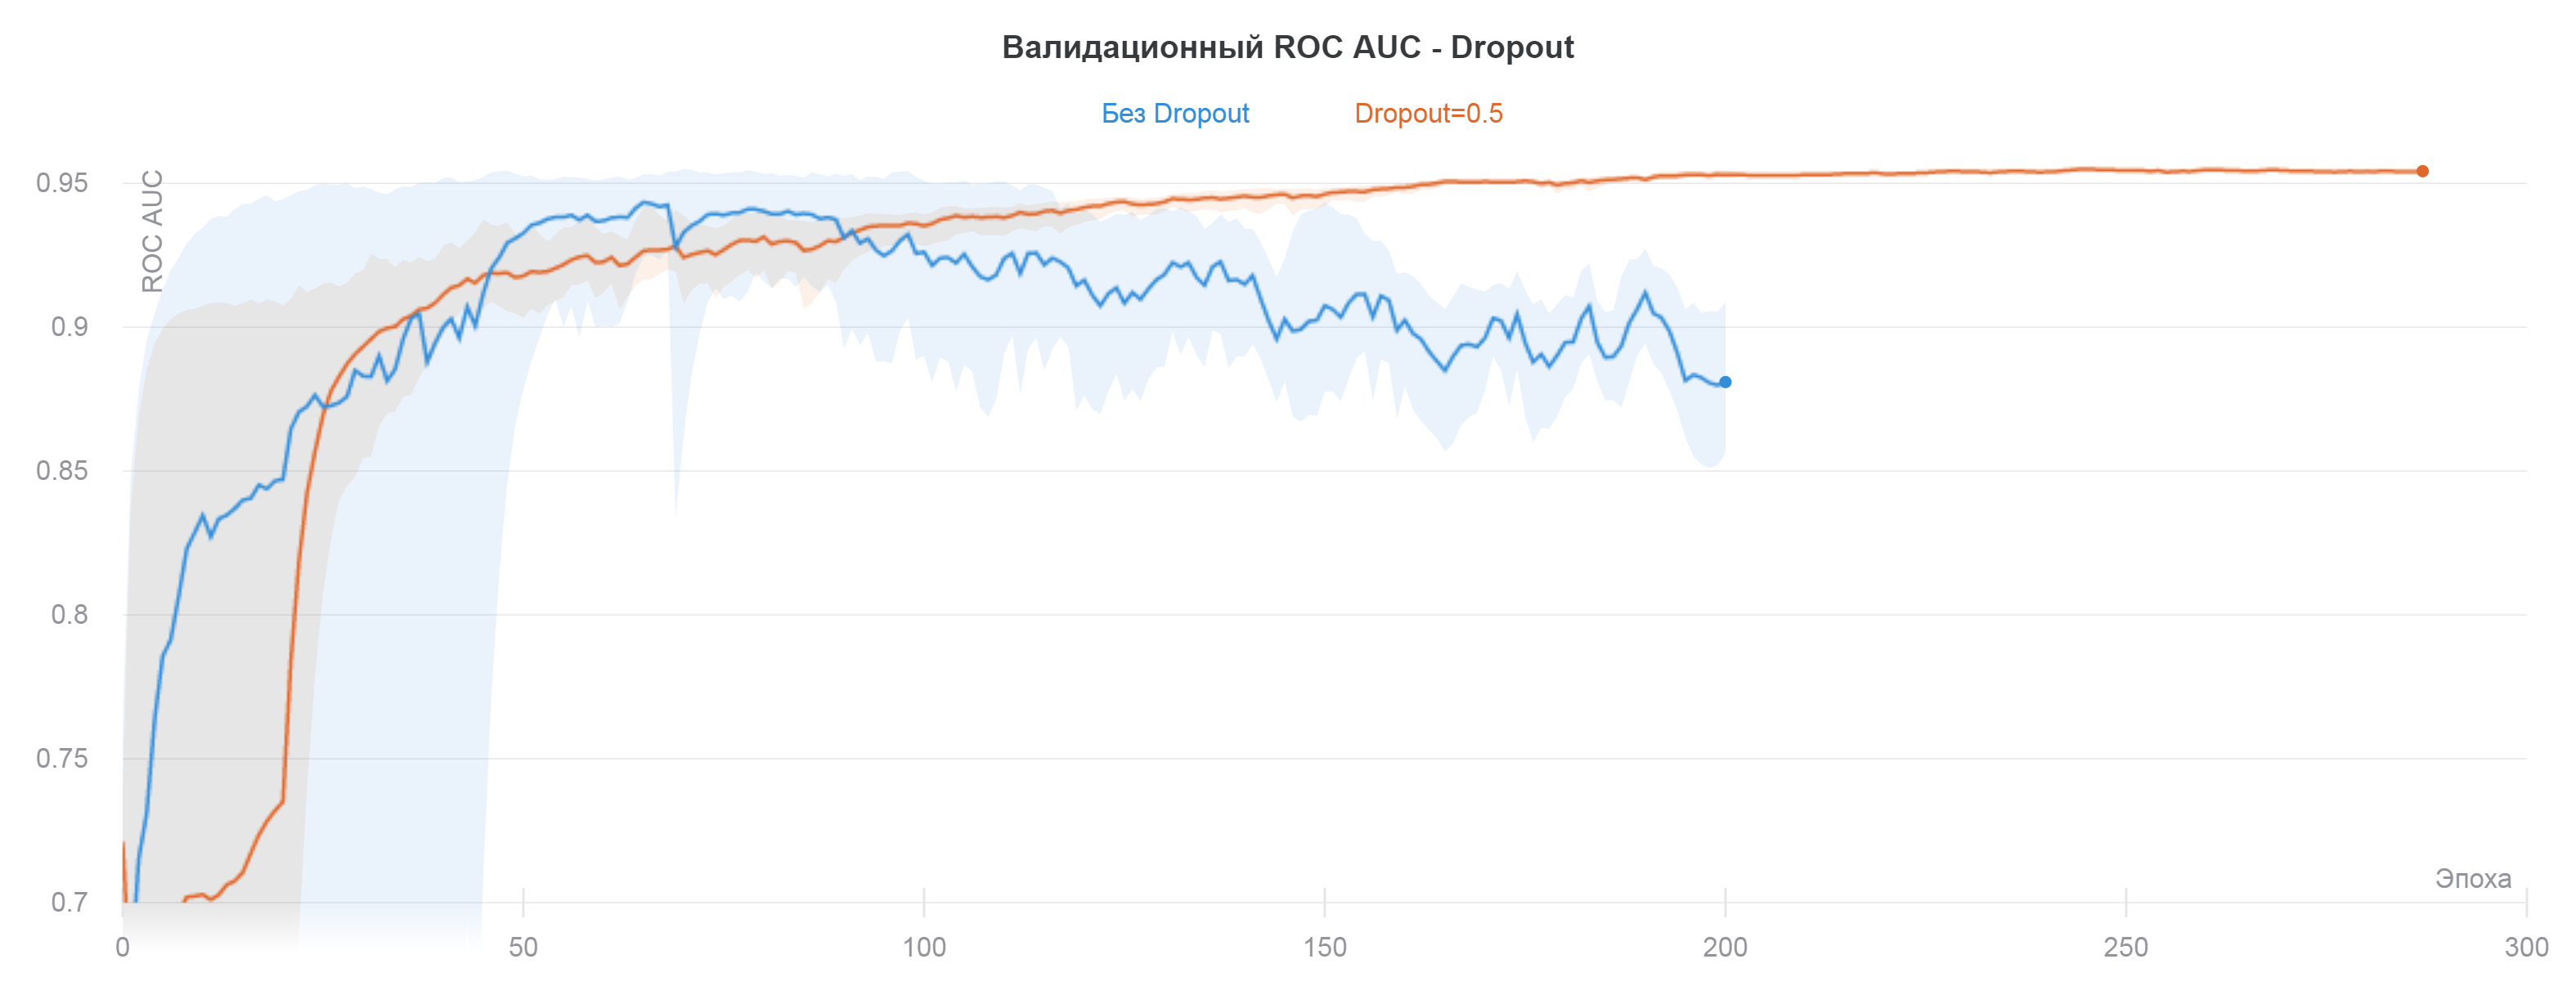
\includegraphics[width=\linewidth]{Section-0-Panel-3-ns9ivtwl4}}
\caption{Сравнение экспериментов с и без применения слоя Dropout}
\label{fig:dropout}

\end{figure}

При добавлении контентных данных, функция потерь у LSTM (\autoref{fig:lstm-loss}) и точность (\autoref{fig:lstm-accuracy}) на валидации несколько улучшаются. Однако, при использовании новых весов LSTM при обучении CNN, ROC AUC на валидации значительно падает.

\begin{figure}[H]

\noindent\makebox[\textwidth]{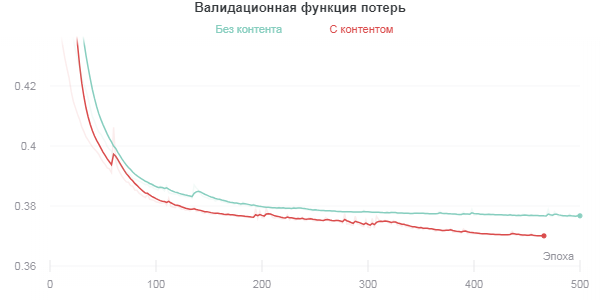
\includegraphics[width=\linewidth]{lstm-loss}}
\caption{Сравнение функции потерь при обучении LSTM с контентом и без}
\label{fig:lstm-loss}

\end{figure}
\begin{figure}[H]
\noindent\makebox[\textwidth]{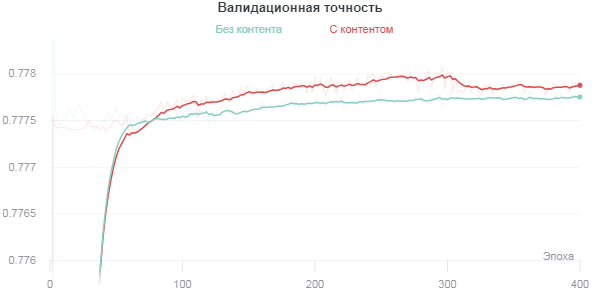
\includegraphics[width=\linewidth]{lstm-accuracy}}
\caption{Сравнение точности при обучении LSTM с контентом и без}
\label{fig:lstm-accuracy}

\end{figure}

Добавление Embedding-слоя в LSTM модель не оказало значимого влияния на качество предсказаний. Было попробовано два варианта обучения с этим слоем: обучение со случайной инициализацией вместе с обучением всей моделей, обучение весов слоя отдельно с помощью модели SkipGram. При обучении весов слоя с помощью SkipGram также есть два варианта: статический (веса Embedding-слоя фиксируются и не меняются при обучении LSTM) и динамический (веса Embedding-слоя дополнительно обучаются вместе с LSTM).\\
В итоге, ни один из вариантов Embedding слоя не улучшил результатов LSTM модели. Среди всех вариантов, статические SkipGram веса показали наилучший результат.
